\documentclass[12pt]{article}
\usepackage[a4paper,margin=0.75in]{geometry}
\usepackage[utf8]{inputenc}
\usepackage[OT1]{fontenc}
\usepackage[table,usenames,dvipsnames]{xcolor}
\usepackage{array}
\usepackage{varwidth}
\usepackage{tabularx}
\usepackage{amsmath}
\usepackage{hyperref}
\usepackage{enumitem}
\usepackage{graphicx}
\usepackage{tcolorbox}
\usepackage{forest}
\usepackage{multirow}
\usepackage{algpseudocode}
\usepackage{parskip}
\renewcommand*\familydefault{\sfdefault}

\newtcolorbox{mybox}[3][]
{
  colframe = #2!25,
  colback  = #2!10,
  coltitle = #2!20!black,  
  title    = {#3},
  #1,
}

\hypersetup{
    colorlinks=true,
    linkcolor=blue,
    filecolor=magenta,      
    urlcolor=cyan,
    %pdfpagemode=FullScreen,
}

\title{\textbf{COL380 Assignment 3}}
\author{%
    \begin{tabular}{c}Aniruddha Deb \\ \texttt{2020CS10869}\end{tabular} \and%
    \begin{tabular}{c}Rishabh Dhiman \\ \texttt{2020CS10837}\end{tabular} %
}
\date{April 2023}

\begin{document}

\maketitle

\section*{Task 1}

\subsection*{Approach}

For this assignment, we changed our algorithm from Hybrid to MinTruss [1], which
was parallelized with inputs from [2]. The core idea is to modify the MinTruss
algorithm by splitting it into phases and using the bulk synchronous parallel
model to synchronize across nodes at the end of each bulk phase. 

The serial algorithm is as follows:
\begin{enumerate}
    \item We start off with triangle enumeration, which is done differently 
        from [2]. We instead precompute all the triangles as is done in [3],
        by ordering the vertices based on their degree and enumerating all
        incident pairs of edges. This runs in $O\left(\sum
        \text{outdeg}(v)^2\right)$
    \item We then use the same algorithm as MinTruss. However, it's implemented
        in a different manner, which involves multiple phases of edge deletion.
        We do this to make it easier to later parallelize the code.
\end{enumerate}

\begin{algorithmic}[1]
    \State Compute initial supports and store in sup;
    \State $k \gets 1$

    \While {$|E| > 0$}
        \State $\mathcal{F}_k \gets \{ e \in E: \text{sup}(e) < k\}$
        \While {$|\mathcal{F}_k| > 0$} 
            \For {$e \in \mathcal{F}_k$} 
                \For {$e' \in \Delta_e$} 
                    \State $\text{sup}(e') \gets \text{sup}(e') - 1$
                \EndFor
                \State $E \gets E \ \{e\}$
                \State $\Gamma(e) \gets k - 1$
            \EndFor
            \State $\mathcal{F}_k \gets \{ e \in E: \text{sup}(e) < k\}$
        \EndWhile
        \State $k \gets k+1$
    \EndWhile
\end{algorithmic}

 We do not use any atomic operations or mutexes on data in the parallel
 algorithm. However, synchronization does happen at the end of each phase. Each
 thread runs lines 6 to 12 concurrently at the end of which the deletions are
 propagated to each thread. In the parallel version, Every vertex and the edges
 incident on it are statically owned by a single virtual thread. We have double the number
 of virtual threads compared to the number of actual threads for load balancing
 reasons: this ensures that our algorithm scales irrespective of how unbalanced
 the initial degree distribution is.

\subsection*{Results}

The program was benchmarked on HPC, using the Skylake nodes. The Intel parallel 
studio 2020 compiler was used as it gave quicker runtimes than GCC, and all
runs were done on testcase 10 of assignment 2: this was chosen as it was
neither too large nor too small, and gave us results in a short time while
still displaying how our program scales to a much larger number of cores.

\begin{figure}[!htbp]
    \centering
    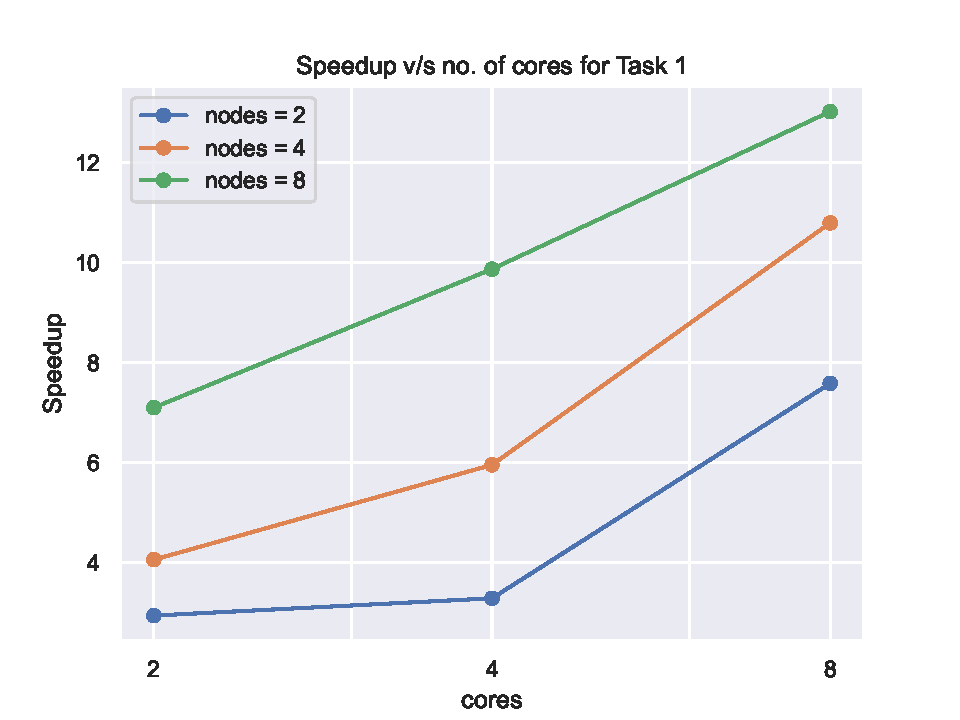
\includegraphics[width=0.48\textwidth]{speedup_t1.pdf}
    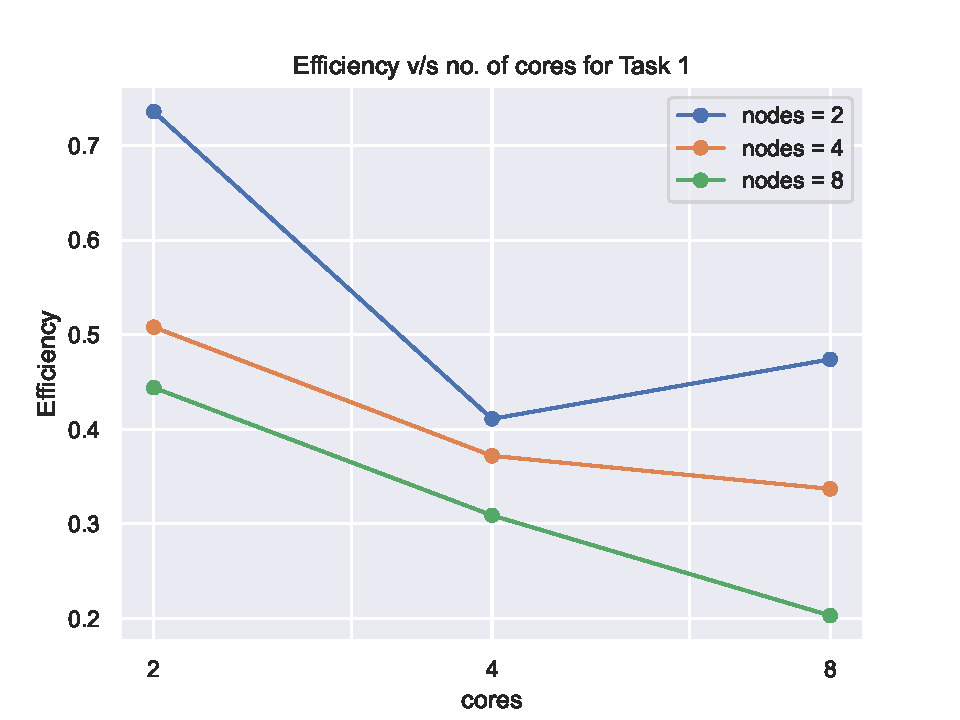
\includegraphics[width=0.48\textwidth]{efficiency_t1.pdf}
\end{figure}

We notice that:
\begin{enumerate}
    \item Efficiency decreases with increasing the number of nodes. This is to 
        be expected, as there is more communication over a higher latency
        network between the nodes compared to shared-memory communication over
        threads
    \item Efficiency also decreases with an increase in the number of threads. 
        This is because of more commmunication between the threads.
    \item The speedup is maximum for 
\end{enumerate}

\begin{table}[!htbp]
    \centering
\begin{tabular}{|c|c|c|c|c|c|}
    \hline
    nodes & threads & speedup & efficiency & isoefficiency & seq. fraction\\

    \hline
    \multirow{3}{*}{2}
    & 2 & 2.943 & 0.736 & 14.331 & 0.119 \\
    & 4 & 3.289 & 0.411 & 57.191 & 0.204 \\
    & 8 & 7.585 & 0.474 & 44.287 & 0.073 \\

    \hline
    \multirow{3}{*}{4}
    & 2 & 4.061 & 0.508 & 38.727 & 0.138 \\
    & 4 & 5.957 & 0.372 & 67.295 & 0.112 \\
    & 8 & 10.795 & 0.337 & 78.415 & 0.063 \\

    \hline
    \multirow{3}{*}{8}
    & 2 & 7.101 & 0.444 & 50.031 & 0.083 \\
    & 4 & 9.872 & 0.309 & 89.487 & 0.072 \\
    & 8 & 13.021 & 0.203 & 156.303 & 0.062 \\
    \hline
\end{tabular}
\caption{Statistics for task 1}
\end{table}

Isoefficiency is lower-bounded by the overhead, and the overhead is given 
by $pt(n,p) - t(n,1)$, which is what we've used here to compute isoefficiency.
The sequential fraction is computed using the formula 
$$f = \frac{\frac{1}{S_p} - \frac{1}{p}}{1 - \frac 1p}$$

The time complexity for our method is roughly given by

$$TC = O\left(\frac{\Delta}{q} + \frac{\sum \text{deg}^+(v)^2}{pq}\right)$$

Where $\Delta$ is the number of triangles in the graph, $q$ is the number of MPI
ranks and $p$ is the number of threads per rank.

\section*{Task 2}

\subsection*{Approach}

Approach 2 is just an extension of approach 1, which first computes a spanning
forest of the k-truss graph on the edges owned by that node. Then we gather all
the edges of the spanning forest on node 0, and compute the spanning forest of 
the entire k-truss graph on node 0. We then broadcast this to all nodes who 
find the influencers based on this and output to a file in a distributed manner
using MPI file IO.

Because of the spanning forest computation on the local nodes, we only need to
send $O(n)$ number of edges while gathering the edges at rank 0 instead of
$O(m)$ edges.

\subsection*{Results}

The evaluation schemes were the same as task 1. The results are given below:

\begin{figure}[!htbp]
    \centering
    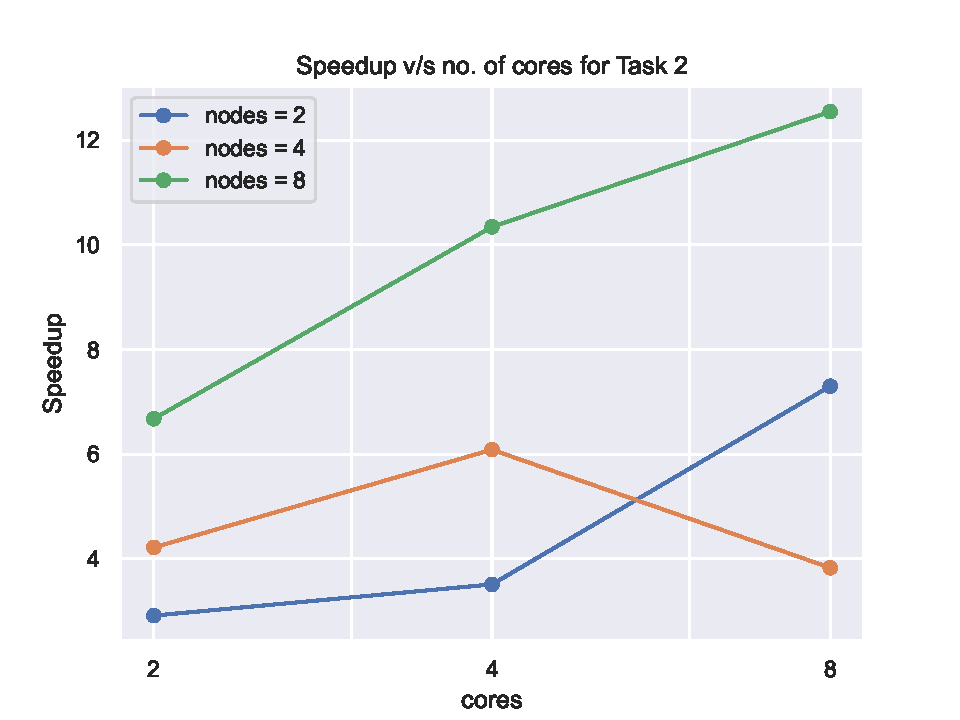
\includegraphics[width=0.48\textwidth]{speedup_t2.pdf}
    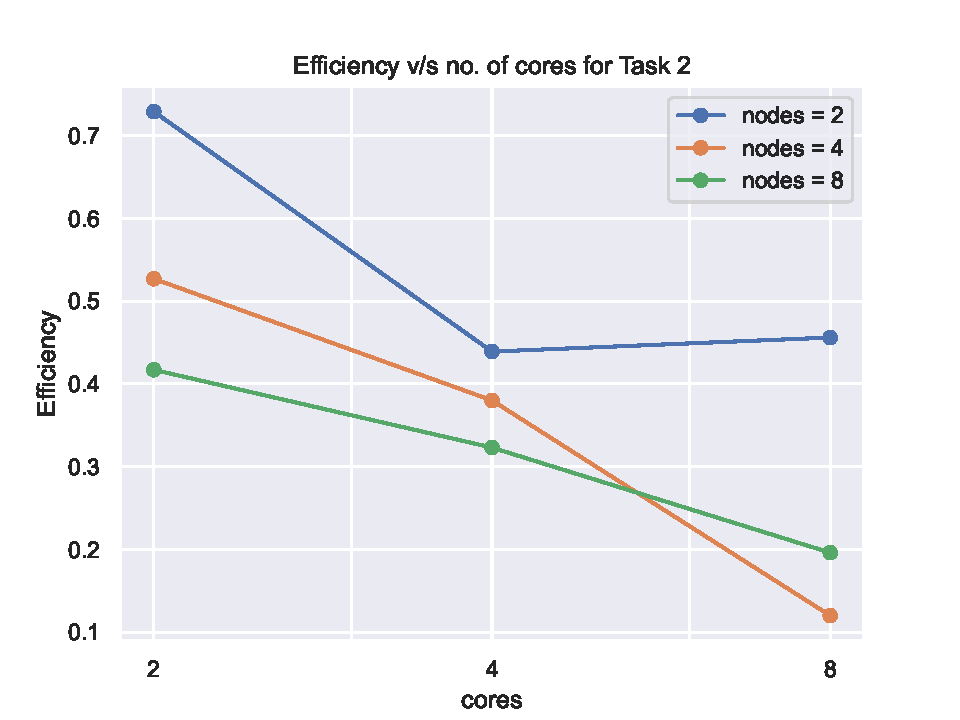
\includegraphics[width=0.48\textwidth]{efficiency_t2.pdf}
\end{figure}

\begin{table}[!htbp]
    \centering
\begin{tabular}{|c|c|c|c|c|c|}
    \hline
    nodes & threads & speedup & efficiency & isoefficiency & seq. fraction\\

    \hline
    \multirow{3}{*}{2}
    & 2 & 2.914 & 0.729 & 14.871 & 0.124 \\
    & 4 & 3.510 & 0.439 & 51.063 & 0.182 \\
    & 8 & 7.298 & 0.456 & 47.599 & 0.079 \\

    \hline
    \multirow{3}{*}{4}
    & 2 & 4.216 & 0.527 & 35.831 & 0.128 \\
    & 4 & 6.085 & 0.380 & 65.055 & 0.108 \\
    & 8 & 3.828 & 0.120 & 82.575 & 0.237 \\

    \hline
    \multirow{3}{*}{8}
    & 2 & 6.676 & 0.417 & 55.759 & 0.093 \\
    & 4 & 10.342 & 0.323 & 83.599 & 0.067 \\
    & 8 & 12.546 & 0.196 & 163.727 & 0.065 \\
    \hline
\end{tabular}
\caption{Statistics for task 2}
\end{table}

The time complexity for this algorithm is 

$$TC = O\left(n\log q + \frac{\Delta}{q} + \frac{\sum \text{deg}^+(v)^2}{pq}\right)$$

Where $n$ is the number of nodes in the graph

\section*{References}

\begin{enumerate}
    \item Cohen, Jonathan. "Trusses: Cohesive subgraphs for social network analysis." \textit{National security agency technical report 16.3.1 (2008)}.
    \item Smith, Shaden, et al. “Truss Decomposition on Shared-Memory Parallel Systems.” \textit{2017 IEEE High Performance Extreme Computing Conference (HPEC), IEEE, 2017}, pp. 1–6. DOI.org (Crossref), \href{https://doi.org/10.1109/HPEC.2017.8091049}{https://doi.org/10.1109/HPEC.2017.8091049}.
\end{enumerate}


\end{document}
